\subsection{Adding Perpendicular to Chains}

\begin{figure}
    \centering
    \begin{subfigure}{0.4\textwidth}
        \centering
        \includegraphics[width=\textwidth]{70_030_SearchAdding_quad2/2D_Period_UpperLeft/result.png}
        \caption{Full}
        %        \label{fig:final.period.whole.full}
    \end{subfigure}
    \begin{subfigure}{0.4\textwidth}
        \centering
        \includegraphics[width=\textwidth]{70_030_SearchAdding_quad2/2D_Period_UpperLeft_Zoomed/result.png}
        \caption{Zoomed-In}
        %        \label{fig:final.period.whole.halved}
    \end{subfigure}
    \caption{2D Scans of Periods of Upper Left Quarter Of Quad2 Model}
\end{figure}

\begin{figure}
    \centering
    \includegraphics[width=0.6 \textwidth]{70_030_SearchAdding_quad2/2D_Regions_UpperLeft_Zoomed/result.png}
    %        \label{fig:final.period.whole.halved}
    \caption{2D Scans of Period Regions in Upper Left Quarter Of Quad2 Model}
\end{figure}

\begin{figure}
    \centering
    \begin{subfigure}{0.4\textwidth}
        \centering
        \includegraphics[width=\textwidth]{70_030_SearchAdding_quad2/1D_Period_UpperLeft_B8_C9/result.png}
        \caption{Between $B_8$ and $C_9$}
        %        \label{fig:final.period.whole.full}
    \end{subfigure}
    \begin{subfigure}{0.4\textwidth}
        \centering
        \includegraphics[width=\textwidth]{70_030_SearchAdding_quad2/1D_Period_UpperLeft_C10_C9/result.png}
        \caption{Between $C_{10}$ and $C_9$}
        %        \label{fig:final.period.whole.halved}
    \end{subfigure}
    \caption{1D Scans of Periods of Upper Left Quarter Of Quad2 Model}
\end{figure}

\begin{figure}
    \centering
    \begin{subfigure}{0.4\textwidth}
        \centering
        \includegraphics[width=\textwidth]{70_030_SearchAdding_quad2/Cobweb_UpperLeft_B8/result.png}
        \caption{At $B_{8}$}
        %        \label{fig:final.period.whole.full}
    \end{subfigure}
    \begin{subfigure}{0.4\textwidth}
        \centering
        \includegraphics[width=\textwidth]{70_030_SearchAdding_quad2/Cobweb_UpperLeft_C10/result.png}
        \caption{At $C_{10}$}
        %        \label{fig:final.period.whole.halved}
    \end{subfigure}
    \caption{Cobwebs at Selected Points of Upper Left Quarter Of Quad2 Model}
\end{figure}